\clearpage
\section{FEM Validation}
\label{AppendixC}

For the stator to be analyzed and redesigned, the Siemens NX program and FEM first have to be validated. This is done with the help of the thin disk problem from assignment 2 \cite{assignment2}.

Consider a thin cylindrical disk with internal radius $R_i$ and external radius $R_o$ as shown in Figure \ref{cylindrical_disk}. The disk is subjected to a temperature $T_i$ on the inner surface and $T_o$ on the outer surface, both defined with respect to some reference temperature, e.g. the ambient temperature. The other disk surfaces are thermally insulated. The disk is mechanically unconstrained, i.e. all surfaces are traction free.

\begin{figure}[H]
\centering
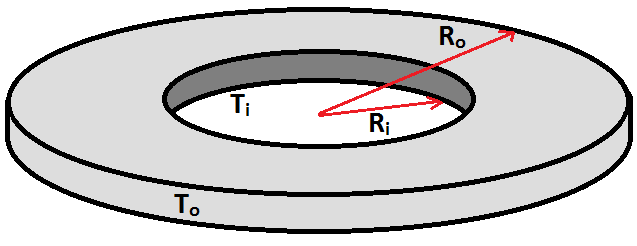
\includegraphics[width=0.5\linewidth]{Figures/kaulovettedisc.png}
\caption{Cylindrical disk}
\label{cylindrical_disk}
\end{figure}
For this problem, both the radial en tangential stress can be expressed analytically:

\begin{equation}
\label{rr}
\sigma_{rr}(r) = \frac{1}{2}E \alpha (\frac{R_{i}^{2}T_{i}(r^{2}-R_{o}^{2})-R_{o}^{2}T_{o}(r^{2}-R_{i}^{2})}{r^{2}(R_{i}^{2}-R_{o}^{2})} + \frac{T_{o}ln(\frac{r}{R_{i}})-T_{i}ln(\frac{r}{R_{o}})}{ln(\frac{R_{i}}{R_{o}})})
\end{equation}

\begin{equation}
\label{theta}
\sigma_{\theta\theta}(r) = \frac{1}{2}E \alpha (\frac{R_{i}^{2}T_{i}(r^{2}-R_{o}^{2})-R_{o}^{2}T_{o}(r^{2}-R_{i}^{2})}{r^{2}(R_{i}^{2} + R_{o}^{2})} + \frac{T_{o}-T_{i}}{ln(\frac{R_{i}}{R_{o}})} + \frac{T_{o}ln(\frac{r}{R_{i}})-T_{i}ln(\frac{r}{R_{o}})}{ln(\frac{R_{i}}{R_{o}})})
\end{equation}

The parameters $T_i$, $T_o$, $R_i$ and $R_o$ are chosen and can be seen in \ref{table:thin_disk}. The material is steel, the according parameters are given as well.\newline
\begin{center}
\begin{table}[H]
\caption{Parameters thin disk}
\begin{center}
\begin{tabular}[c]{|l|l|l|}
\hline
\label{table:thin_disk}
What & Value & Unit\\
\hline
$T_i$ & $300$ & \textdegree{}C\\
$T_o$ & $100$ & \textdegree{}C\\
$R_i$ & $150$ & $mm$\\
$R_o$ & $85$ & $mm$\\
$E$ & $206.94\cdot 10^9$ & $Pa$\\
$\alpha$ & $1.128\cdot 10^{-5}$ & $1/$\textdegree{}C \\
$d$ & $5$ & $mm$\\
\hline
\end{tabular}
\end{center}

\end{table}
\end{center}


The parameters are the exact same as the ones that were used in assignment 2. However now the thin disk is used to check the validity of the FEM software. This is done by checking the max tangential stress in the thin disk determined numerically  and comparing this to the max tangential stress that is determined analytically, see figure \ref{fig:Ass2NumVsAna}. See Appendix \ref{AppendixB} for the solution of assignment 2. 

\begin{figure} [H]
	\centering
	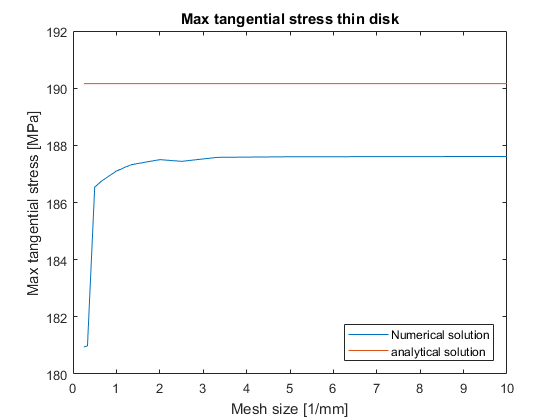
\includegraphics[width=0.8\linewidth]{Figures/Numerical_Analytical_Tangential.png}
	\caption{Comparison numerical and analytical solution}
    \label{fig:Ass2NumVsAna}
\end{figure}

In this figure it is clear that the numerical solution levels out around 187.61 [MPa] (See Appendix \ref{AppendixB}. Whereas the analytical result is equal to 190.16 [MPa]. This means that there is a $\pm$2.5 [MPa] difference between the FEM analysis and the analytical solution. It also shows that the mesh of 2 [mm] is already pretty close to the final stress of the finest mesh and from 0.5 [mm] onward there is no significant difference anymore in smaller mesh sizes.


So what do these results say about the accuracy of FEM analysis. The difference of 2.5 [MPa] seems like a very big difference, but when it is looked at as a percentage of the whole stress spectrum, it is only equal to 0.56\%. This means that NX has an inaccuracy of at least 0.56\%.




% \begin{figure} [H]
% 	\centering
% 	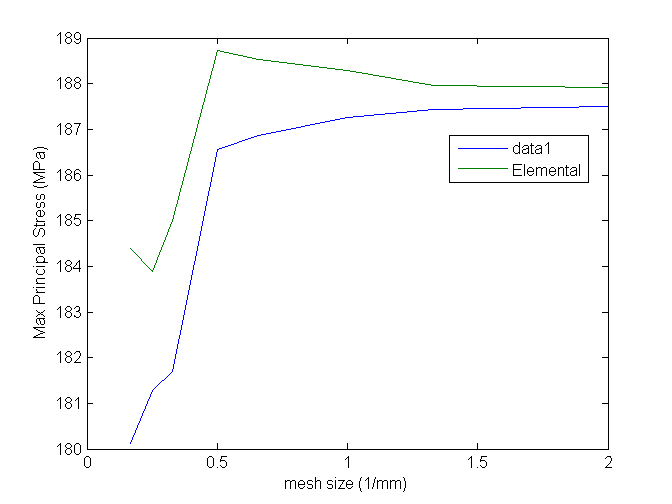
\includegraphics[width=0.8\linewidth]{Figures/convergence.png}
% 	\caption{Convergence}
%     \label{fig:Ass2Convergence}
% \end{figure}

